\documentclass{beamer}
\usepackage{amsmath}
\usepackage{graphicx}
\usepackage{cite}
\usepackage{tikz}
\usepackage{amsmath}
\usepackage{graphicx}
\usepackage{tikzit}

\usepackage{xcolor}

\definecolor{myred}{RGB}{255, 0, 0}
\definecolor{myyellow1}{RGB}{255, 255, 219}
\definecolor{mygreen1}{RGB}{0, 255, 0}
\definecolor{mygreen2}{RGB}{0, 126, 0}
\definecolor{myblue}{RGB}{0, 0, 255}

\usetikzlibrary{arrows.meta,positioning}
\usetikzlibrary{shapes.multipart,matrix,positioning,arrows,arrows.meta}
\usefonttheme{serif}
\input{sample.tikzstyles}
% Edge styles

\setbeamertemplate{footline}[frame number]{}
\setbeamertemplate{navigation symbols}{}

\usecolortheme{lily}
\setbeamercolor{block title}{bg=blue!20,fg=black}
\setbeamercolor{block body}{bg = blue!10, fg = black}
\setbeamertemplate{itemize item}[square]
\setbeamercolor{itemize item}{fg = cyan}
\setbeamercolor{enumerate item}{fg = cyan}

\usetheme{default}
\beamertemplatenavigationsymbolsempty
\setbeamercolor{titlelike}{fg=blue}
\setbeamertemplate{caption}{\insertcaption\par}

%Information to be included in the title page:
\title{Characterizing evolutionary dynamics on a broader scale: a strain-space model for SARS-CoV-2}
\author{Peter C. Jentsch, PhD \inst{1,4} \and Finlay Maguire, PhD  \inst{3,5} \and Samira Mubareka, MD, FRCPC \inst{1,2}}
\institute{\inst{1} Sunnybrook Research Institute, Toronto, Canada  \and \inst{2} University of Toronto, Toronto, Canada \and \inst{3} Dalhousie University, Halifax, Canada \and \inst{4} Simon Fraser University, Burnaby, Canada \and \inst{5} Shared Hospital Laboratory, Toronto, Canada}
\date{\today}

\begin{document}
\setbeamertemplate{caption}{\insertcaption\par}


\begin{frame}{Projecting to low dimensions while preserving distances}

    Let $D$ be the matrix of measured pairwise distances. 

    Multidimensional scaling (MDS) finds $x_i \in \mathbb{R}^k$ to minimize 
    \[ 
        \text{STRESS}(\boldmath{x}) = \sum_{i>j} \left(D_{ij} - \lVert x_i - x_j \rVert\right)^2
    \]

    where $k$ is small.

    \begin{columns}
        \begin{column}{0.4\textwidth}
            \begin{figure}
                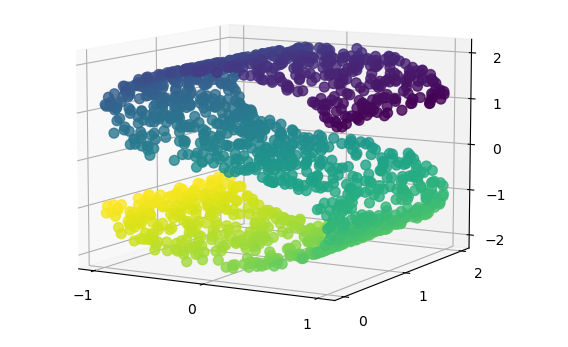
\includegraphics[width=1.4\textwidth]{standalone/mds_1.png}
                
            \end{figure}   
        \end{column}
        \begin{column}{0.01\textwidth}
            \huge{$\Longrightarrow$}
            
        \end{column}
        \begin{column}{0.4\textwidth}
            \begin{figure}
            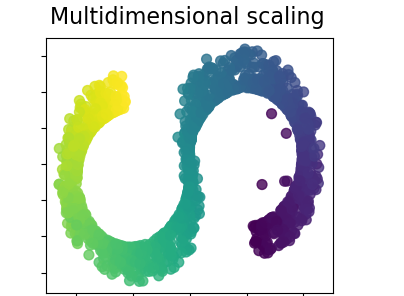
\includegraphics[width=\textwidth]{standalone/mds_2.png}
        \end{figure}   
        \end{column}
    \end{columns}
    \centering
    \tiny{\cite{scikit-learn}}
\end{frame}


\begin{frame}{Bayesian MDS}
    \begin{itemize}
        \item Want to specify priors for $x_i$
        \item First published by Oh and Raftery \cite{oh2001bayesian}
        \item Let $D$ be the matrix of measured distances between points
        \item Assumes \[ D_{ij} \sim N(\lVert x_i - x_j \rVert,\sigma^2)I(D_{ij} > 0) \]
        \item where $x_i \in \mathbb{R}^k$
        \item Estimate parameters with Markov Chain Monte Carlo (MCMC) methods 
        \item Extremely computationally expensive!
    \end{itemize}
\end{frame}

\begin{frame}{MassiveMDS: an OpenCL implementation of likelihood and gradient functions for MDS}
    \begin{figure}
        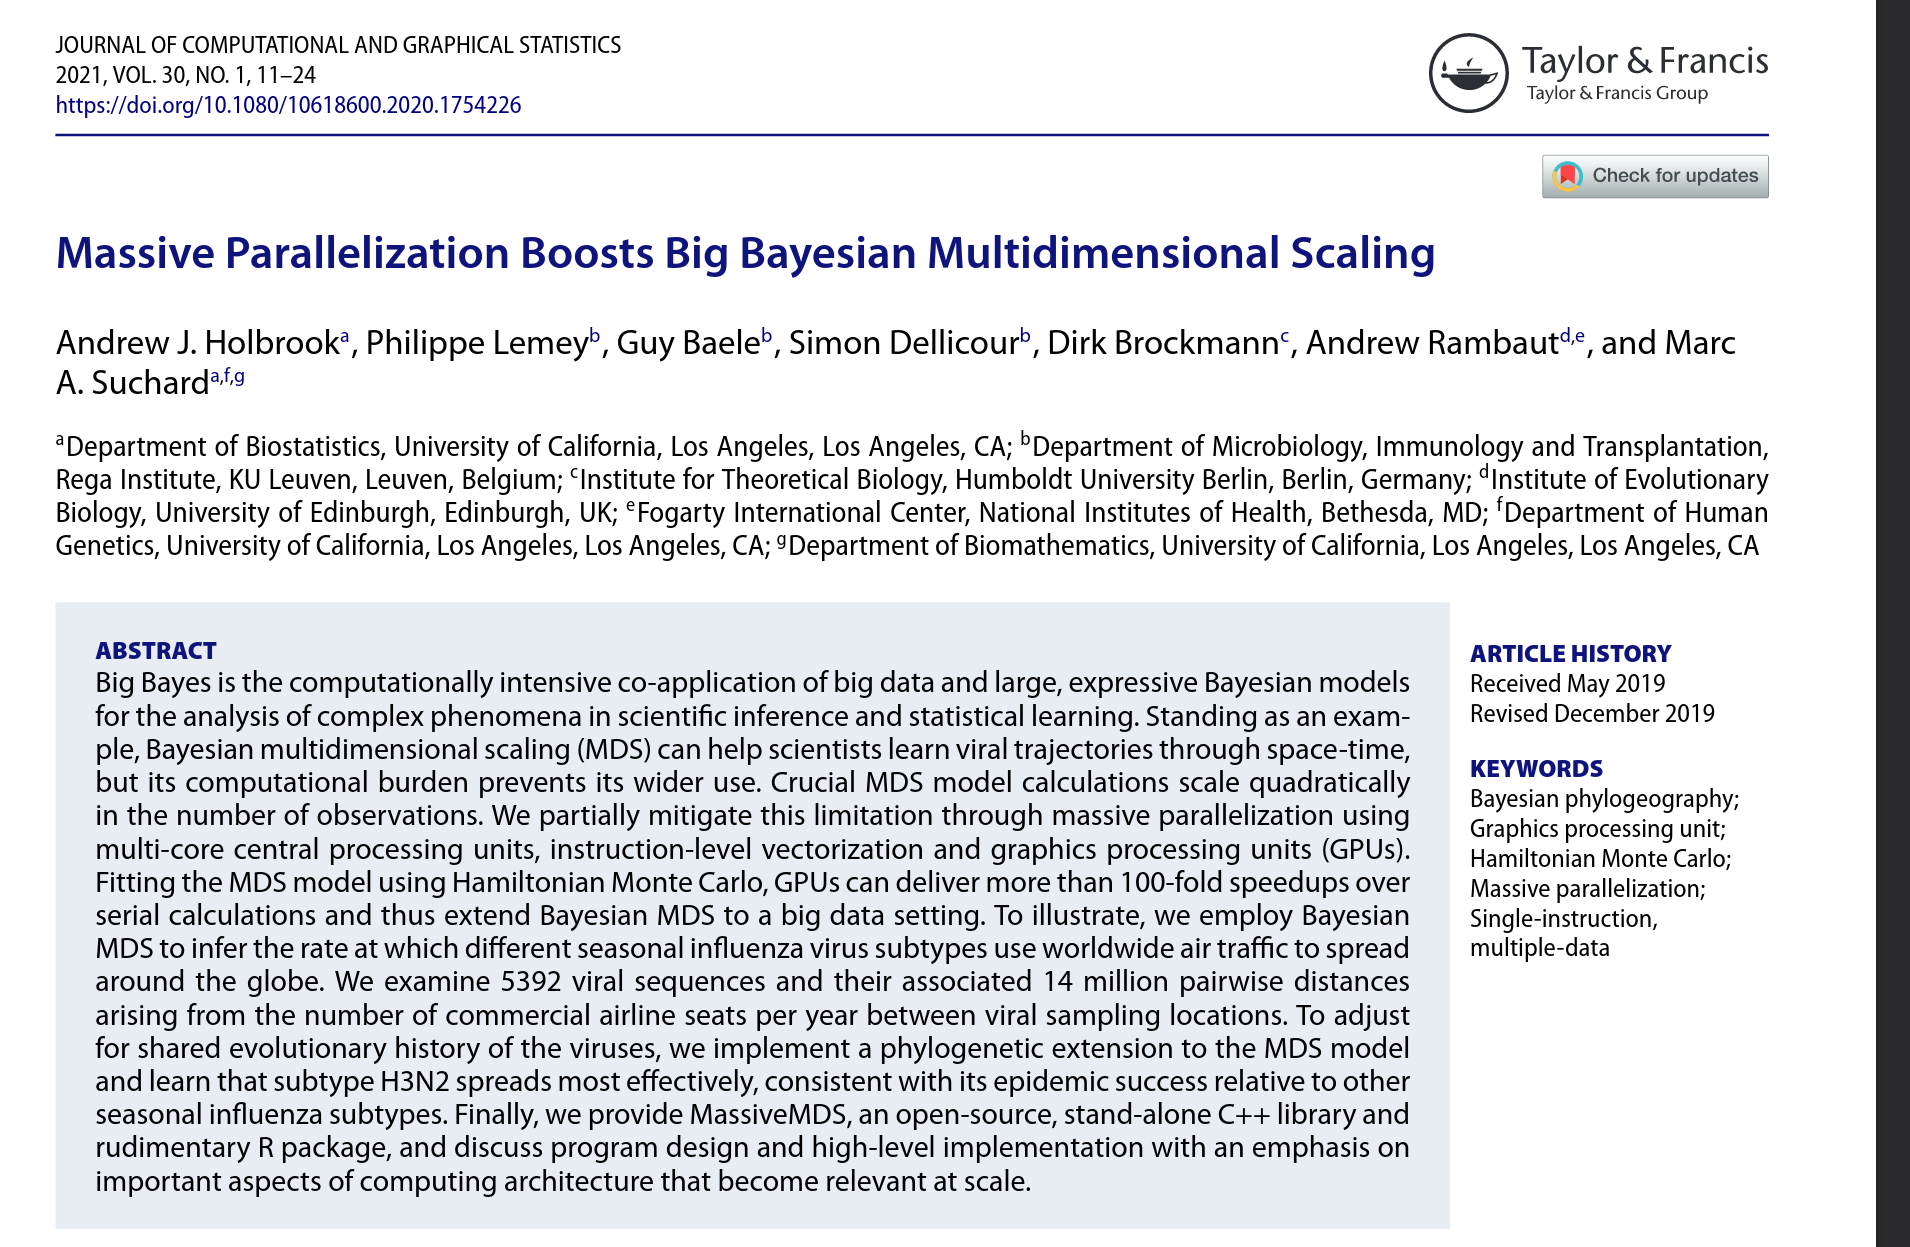
\includegraphics[width=1.0\textwidth]{2022-10-03-21-17-16.png}
    \end{figure}   
\end{frame}

\begin{frame}{Some questions I still have}
    \begin{itemize}
        \item The code contains a lot of fitting ``precision" of the MDS likelihood, but nothing in the paper about this. Is this referring to the float precision used to compute the likelihood?
        \item There are also mentions of learning traits in the code but not the paper, which I think has to do with the integration of this package to BEAST
    \end{itemize}
\end{frame}

\begin{frame}[allowframebreaks]

\bibliographystyle{apalike}
\bibliography{ref.bib}
\end{frame}
\end{document}